\documentclass[../ProgettoTecWeb2.tex]{subfiles}

\begin{document}
\section{La ricerca}
	Come fatto già notare, il sito offre uno strumento per la ricerca. Dal momento che il sito comprende più di 1000 pagine tale scelta è fondamentale poichè, altrimenti, un utente non avrebbe modo di cercare i contenuti che più gli interessano. Il sito non si avvale del tool messo a disposizione da Google, ma è stata implementata una ricerca locale che, a mio parere, funziona sufficientemente bene. \\
	Lo strumento si presenta con un box di ricerca in cui un utente può inserire del testo di lunghezza 60 caratteri, prima che si presenti lo scroll orizzontale. Questa lunghezza è ottimale pensando che il 90\% degli utenti è soddisfatto con un box di 30 caratteri e che il box di ricerca di Google è di 63 caratteri. \\
	La barra di ricerca, però, non è sempre visibile ma appare solamente dopo un click sull'icona rappresentante la lente di ingrandimento. Tale scelta, sempre più utilizzata e proveniente dal mondo del mobile, non è la migliore: gli utenti infatti preferiscono ancora vedere il bottone con il testo ``Cerca'', rispetto che le icone. Tale scelta può essere giustificata pensando al pubblico a cui è diretto il sito web: giovani o comunque persone che hanno una certa dimestichezza con computer, console per videogiochi e videogiochi e quindi, presumibilmente, anche con le interfacce dei dispositivi mobile. Potrebbe essere preferibile lasciare visibile la barra di ricerca visibile, in modo tale da non obbligare l'utente a fare un click in più. Inoltre vi è lo spazio sufficiente per fare ciò senza rovinare il layout. \\
	Può essere discutibile la scelta del placeholder utilizzato che recita ``Premi invio per cercare...''. Preferibile sarebbe inserire un suggerimento, un esempio oppure una semplice scritta ``Cerca...''.
	\begin{figure} [H]
		\centering
		
\includegraphics[scale=0.3]{img/BarraMenuILoveVg}
		\caption{Barra del menù prima del click sull'icona della ricerca}
	\end{figure}
	\begin{figure} [H]
		\centering
		
\includegraphics[scale=0.3]{img/BarraMenuILoveVgDopoClick}
		\caption{Barra del menù dopo il click sull'icona della ricerca}
	\end{figure}

	\subsection{L'esposizione}
	La pagina con i risultati di una ricerca che abbia prodotto risultati è molto simile alle pagine delle news, recensioni, etc. e ne presenta pregi e difetti. 
	Viene anche in questo caso utilizzata la visualizzazione a griglia. Come accennato tale tipo di esposizione fa perdere tempo agli utenti perché c'è un grado di libertà troppo ampio per l'ispezione dei risultati e ciò richiede un tempo ed uno sforzo maggiore. Inoltre, se si volesse dare una classifica di importanza ai risultati, questo non sarebbe possibile.
	Nella pagina con i risultati troviamo in alto riportato ciò che abbiamo cercato con la possibilità di applicare il filtro per effettuare la ricerca solamente tra le news, tra le recensioni, tra le anteprime oppure tra i contenuti speciali.
	\begin{figure} [H]
		\centering
		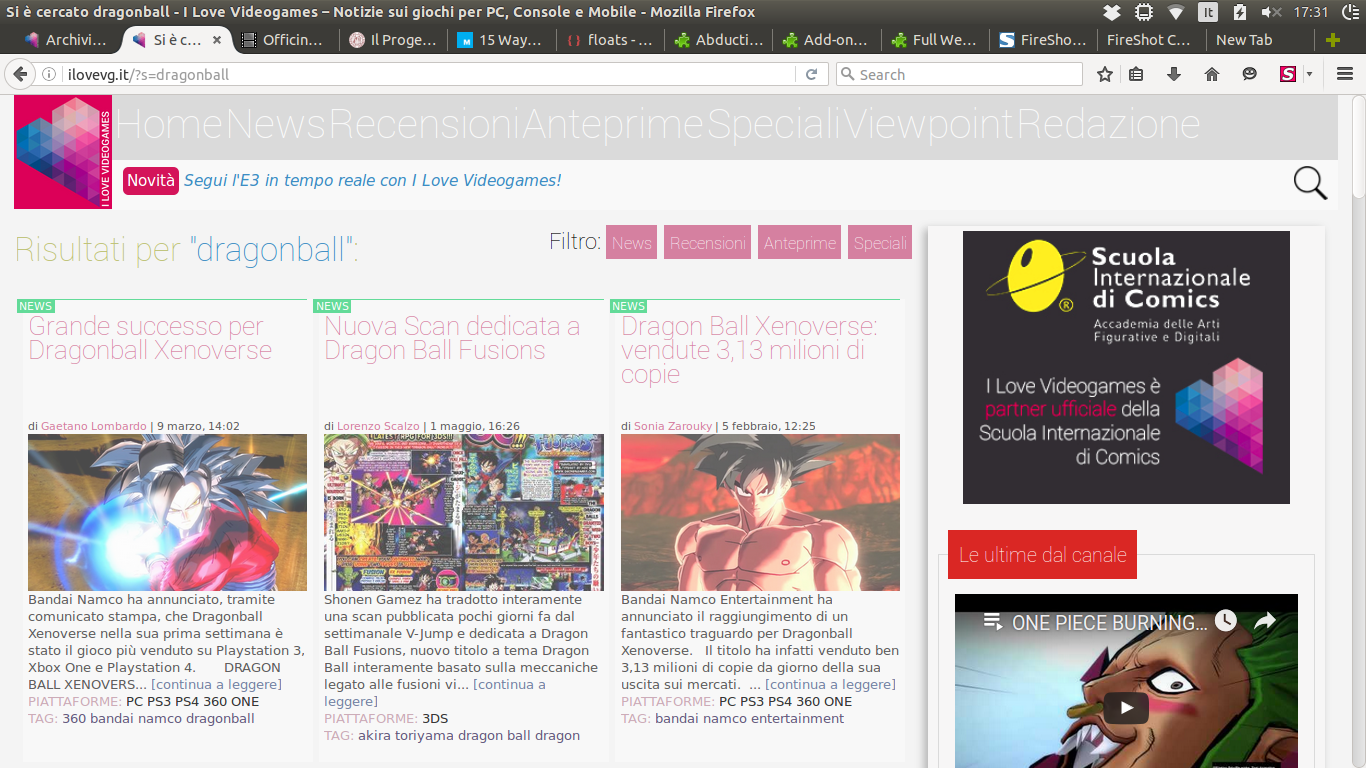
\includegraphics[scale=0.2]{img/RicercaConRisultati}
		\caption{Pagina dei risultati cercando ``dragonball''}
	\end{figure}

	Nel caso in cui la ricerca non produca alcun risultato invece viene visualizzata una pagina che spiega appunto che ciò che è stato cercato non è associato ad alcun contenuto del sito.
	\begin{figure} [H]
		\centering
		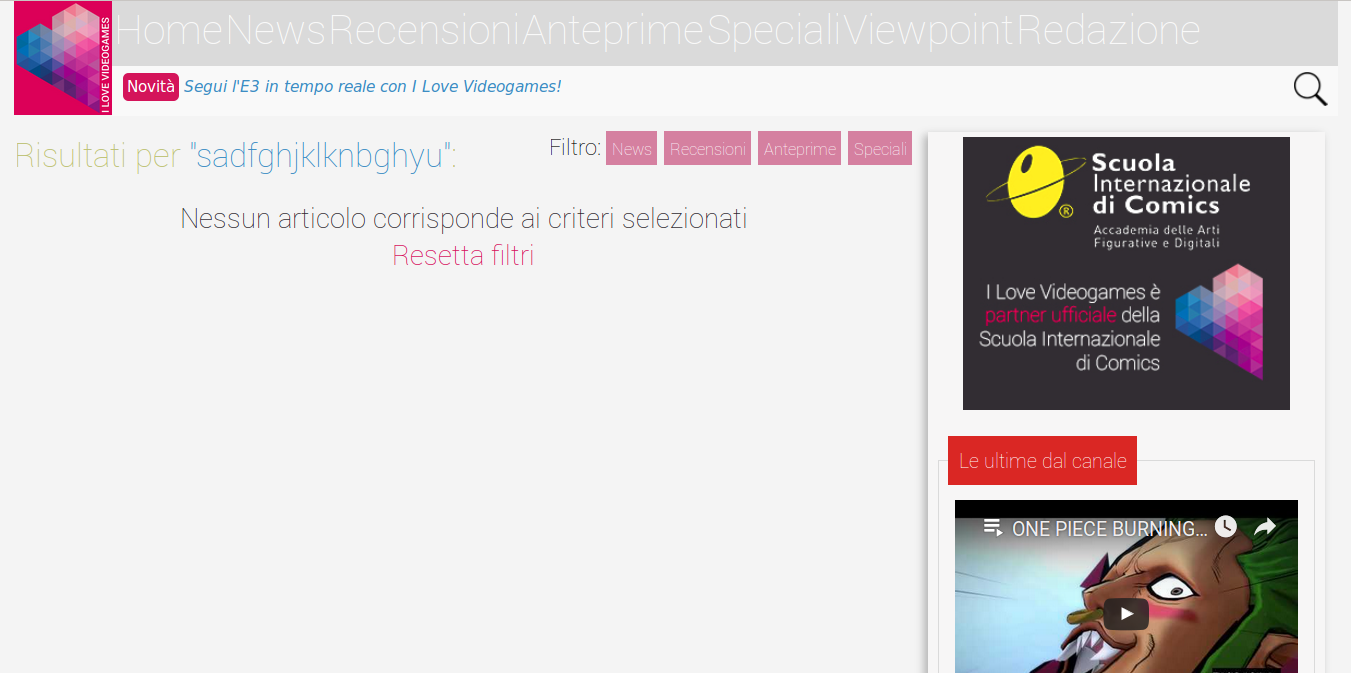
\includegraphics[scale=0.2]{img/RicercaNoRisultati}
		\caption{Pagina dei risultati cercando ``sadfghjklknbghyu''}
	\end{figure}

\end{document}